%%%%%%%%%%%%%%%%%%%%%%%%%%%%%%%%%%%%%%%%%%%%%%%%%%%%%%%
% 10/09/06 [Jan]: lay-out, foutjes verbeterd, figuren toegevoegd
%
% 28/06/06 [Greetje]: verbeteringen
% 15/O6/O6 [Roos]: aanpassingen stappenplan: definitie schakelfunctie=2-waardige Boolse functie: extra oef 6 Karnaugh met overlappingen:
% 3/5/04 [Jan]: storende fout verbeterd (fout: a+1=a; juist: a+1=1)
%
% 19/9/02 [Jan]: Aanpassingen op basis van opmerkingen van
%	Greet en Roos. Bijvoegen van een quote vooraan.
%
% 1/7/02 [Jan]: aangemaakt op basis van een wordperfect
%	tekst van verschillende academiejaren terug.
% 08/06 aanpassingen greetje en roos
%%%%%%%%%%%%%%%%%%%%%%%%%%%%%%%%%%%%%%%%%%%%%%%%%%%%%%%%

%% R van re�le getallen (te gebruiken in math-omgeving)
\newcommand{\R}{\mathrm{I}\!\mathrm{R}}

\chapter{Propositielogica en Boolse Algebra}
\begin{quote}
    \textit{{\small Alice had met enige nieuwsgierigheid over zijn
    schouder gekeken. `Wat een grappig horloge!' merkte ze op. `Het
    geeft de dag van de maand aan, maar niet hoe laat het is!'}}

    \textit{{\small `Moet dat dan? mopperde de Hoedenmaker. `Heb jij
    een horloge dat het jaar aangeeft?'}}

     \textit{{\small `Natuurlijk niet', antwoordde Alice prompt, `maar
     dat is omdat het een hele tijd hetzelfde jaar blijft.'}}

     \textit{{\small `\emph{Dat} is met het mijne net zo,' zei de Hoedenmaker.}}


          Uit `Alice in Wonderland' -- Lewis Carroll
\end{quote}
\newpage

Een essentieel onderdeel van elk algoritme --- behalve misschien de allereenvoudigste algoritmes --- is de mogelijkheid om te bepalen welke stap er moet gezet worden op basis van het antwoord op een vraag. De eenvoudigste vraag is de ja/nee vraag: Regent het? Is het vandaag woensdag? We spreken bij een programma over \emph{testen}. Vele programmeertalen kennen hiervoor trouwens een speciaal type variabele\footnote{Bij een aantal talen kent men bijvoorbeeld het type `boolean' met als mogelijke waarden `true' en `false'.}.

We kunnen testen combineren of uitbreiden met voegwoorden zoals \emph{niet}, \emph{en}, \emph{of}, waardoor de mogelijkheden enorm toenemen. Vaak neemt echter de complexiteit van dergelijke samengestelde testen ook toe. In dit hoofdstuk onderzoeken we of dergelijke ingewikkelde testen niet kunnen vereenvoudigd worden. Dit kan door middel van rekenwerk, maar dat is niet altijd de meest geschikte weg. Daarom bekijken we een grafische vereenvoudigingstechniek die gebruik maakt van zogenaamde Karnaugh-afbeeldingen.

\section{ Propositielogica}
 \subsection{Proposities}
 \subsubsection{Definitie}
Een \emph{propositie} of \emph{uitspraak} is elke zin waarvan kan worden gezegd of hij waar of onwaar is.

\subsubsection{Voorbeelden}
%%%%puntkomma's toegevoegd
\begin{itemize}
  \item Rome is de hoofdstad van Itali\"{e};
  \item 2 is een deler van 123;
  \item Er bestaat een getal dat strikt positief en strikt negatief is;
  \item Als de zon schijnt, dan ga ik wandelen;
  \item Alle getallen zijn even of oneven.
\end{itemize}

\subsubsection{Tegenvoorbeelden}
%%%%% lay-out wat veranderd
\begin{itemize}
  \item $2x + 3 = 0$ \\(is niet te controleren op het waar zijn);
  \item Driehoek ABC is rechthoekig \\(over welke driehoek gaat het hier?);
  \item \fbox{De omkaderde zin is vals.}  \\Hier kan de waarheid van de zin niet worden nagegaan omdat (1) als de omkaderde zin onwaar (vals) is, dit tegelijkertijd betekent dat de zin ``de omkaderde zin is vals'' onwaar moet zijn, dus (2) is de omkaderde zin waar. In onze logica kan een zin nooit \emph{tegelijkertijd} waar en onwaar zijn.
\end{itemize}

\subsubsection{Enkelvoudige en samengestelde uitspraken}
\emph{Samengestelde} uitspraken zijn d.m.v. voegwoorden uit \emph{enkelvoudige} uitspraken opgebouwd. De belangrijkste voegwoorden zijn: `en', `of', `als ... dan', `niet' en `als en alleen als' (of de talloze varianten die het Nederlands rijk is).
\subsubsection{Notaties}
We gebruiken de letters $p, q, r, \ldots$ voor de uitspraken en geven ze de naam `propositieveranderlijken'. Voor de voegwoorden gebruiken we de symbolen uit tabel~\ref{tbl:voegwoorden}.


\begin{table}[htb]
  \centering
\begin{tabular}{|c|c|c|}
\hline
 symbool  & betekenis & benaming \\ \hline \hline
  $\en$ & en & conjunctie \\
   $\of$ & of & disjunctie \\
   $\niet$ & niet & negatie \\
   $\alsdan$ & als \ldots dan & implicatie \\
   $\asa$ & als en slechts als & equivalentie \\
\hline
\end{tabular}
  \caption{De vijf belangrijkste voegwoorden}\label{tbl:voegwoorden}
\end{table}

\subsubsection{Formule}
Een \emph{formule} is een zinvolle uitdrukking opgebouwd uit veranderlijken, voegwoorden en haakjes,
bvb. \ $F = \niet (p \en q) \alsdan (\niet r \of p)$

\subsubsection{Voorrangsregels}
In volgorde van hoog naar laag: $\niet \en \of \stackrel{\alsdan}{\asa}$. Dit wil bvb.\ zeggen dat je de formule  $p \alsdan q \of r$ moet lezen als $p \alsdan (q \of r)$ , en \emph{niet} als $(p \alsdan q) \of r$.

\subsection{Waarheidstabellen}
  \subsubsection{Het begrip waarheidswaarde}
Voor elke uitspraak zijn er 2 mogelijkheden: ze is waar, of ze is onwaar. Met elke propositieveranderlijke $p$ associ\"{e}ren we zijn waarheidswaarde $w(p)$. We spreken af:
\begin{displaymath}
%%%% puntkomma toegevoegd
\begin{array}{rl }
    w(p)  & = 1 \mbox{, als de uitspraak } p \mbox{ waar is };  \\
      &  = 0 \mbox{, als de uitspraak } p \mbox{ onwaar is.}
\end{array}
  \end{displaymath}
We geven deze gegevens weer in een \emph{waarheidstabel}. Voor twee proposities $p$ en $q$ hebben we 4 mogelijke combinaties, weergegeven in tabel~\ref{tbl:waarheid}.
\begin{table}[htb]
  \centering
\begin{tabular}{|c|c|}
\hline
$p$  & $q$  \\ \hline \hline
0  & 0  \\
0  & 1 \\
1  & 0 \\
1  & 1 \\
\hline
\end{tabular}
  \caption{Mogelijke combinaties voor twee propositieveranderlijken}\label{tbl:waarheid}
\end{table}
\noindent
Algemeen heeft een waarheidstabel met $n$ veranderlijken $n$ kolommen en $2^{n}$ rijen (zie ook verder).

\subsubsection{De waarheidswaarde van de 5 voegwoorden}
We defini\"{e}ren de waarheidswaarde van de 5 voegwoorden via de waarheidstabel (tabel~\ref{tbl:waarheidvoegwoorden}). De waarheidswaarde van een samengestelde uitspraak hangt af van de waarheidswaarde van de samenstellende elementaire uitspraken.

\begin{table}[htb]
  \centering
\begin{tabular}{|c|c|c|c|c|c|c|}
\hline
 $p$  & $q$ & $\niet p$ & $p \en q$ & $p \of q$ & $p \alsdan q$ & $p \asa q$ \\
\hline \hline
  0 & 0 & & 0 & 0 & 1 & 1\\
  0 & 1 & 1 & 0 & 1 & 1 & 0\\
  1 & 0 & 0 & 0 & 1 & 0 & 0\\
  1 & 1 &  & 1 & 1 & 1 & 1\\
\hline
\end{tabular}
  \caption{Waarheidswaarde van samengestelde uitspraken}\label{tbl:waarheidvoegwoorden}
\end{table}

\subsubsection{Oefening}
Onderzoek de waarheidswaarde van de formule $f = (\niet p \of q) \alsdan (r \en p)$.\\

%%%%%Verandering Greetje
\subsubsection{Oplossing: Waarheidstabel opstellen}
Hoe stel je op een systematische manier de waarheidstabel van de formule $f$ op? We bepalen eerst welke kolommen er zijn en vervolgens het aantal rijen van de tabel.

We maken in de waarheidstabel een kolom voor elke variabele, de samenstellende onderdelen en ten slotte de gehele formule. De formule bevat 3 veranderlijken ($p$, $q$ en $r$). Haar samenstellende onderdelen zijn achtereenvolgens $\niet p$, $\niet p \of q$, $r \en p$. De tabel bestaat bijgevolg uit 7 kolommen (zie tabel~\ref{tbl:oefdrievar}).

Het aantal rijen is gelijk aan $2^3=8$.  De formule bevat immers 3 veranderlijken ($p$, $q$ en $r$). Elk van deze veranderlijken kan twee waarden hebben (0 en 1). De drie veranderlijken zijn onafhankelijk van elkaar. Voor elke veranderlijke zijn er 2 mogelijkheden. Het totaal aantal mogelijke combinaties\footnote{In kansrekenen spreekt men over de \emph{productegel}} van de veranderlijken bedraagt dus $2 \cdot 2 \cdot 2 = 8$. Elk van de drie veranderlijken $p$, $q$ of $r$ zal dus 4 keer de waarde 0 en 4 keer de waarde 1 hebben.

De rijen van de tabel worden niet in een willekeurige volgorde geplaatst. Voor de $p$-kolom groeperen we de nullen en de enen per 4. Voor de $q$-kolom is er om de twee regels een afwisseling tussen 0 en 1. Voor de $r$-kolom wisselen 0 en 1 om de regel af. Ga zelf na dat je op die manier het binaire equivalent van de getallen van 0 t.e.m.\ 7 bekomt voor $pqr$.
\begin{table}[htb]
  \centering
\begin{tabular}{|ccc|cccc|}
\hline
 $p$  & $q$ & $r$ & $\niet p$ & $\niet p \of q$ & $r \en p$ & $\mbox{formule } f$ \\
 %%%%% Tot hier verandering (!spatie na formule)
\hline \hline
0 & 0 & 0 & 1 & 1 & 0 & 0 \\
0 & 0 & 1 & 1 & 1 & 0 & 0 \\
0 & 1 & 0 & 1 & 1 & 0 & 0 \\
0 & 1 & 1 & 1 & 1 & 0 & 0 \\
1 & 0 & 0 & 0 & 0 & 0 & 1 \\
1 & 0 & 1 & 0 & 0 & 1 & 1 \\
1 & 1 & 0 & 0 & 1 & 0 & 0 \\
1 & 1 & 1 & 0 & 1 & 1 & 1 \\
\hline
\end{tabular}
  \caption{Waarheidstabel voor $f=(\niet p \of q) \alsdan (r \en p)$}\label{tbl:oefdrievar}
\end{table}

\subsection{Tautologie\"{e}n of wetten}
\subsubsection{Definities}
%%%%%titel toegevoegd owv uniformiteit elders
Een formule of uitspraak\footnote{We gebruiken beide begrippen min of meer als synoniemen. Bij \emph{uitspraak} denken we eerder in termen van taal, terwijl we bij het begrip \emph{formule} eerder symbolen (letters, veranderlijken) zullen gebruiken.} die \emph{waar} is \emph{on}afhankelijk van de waarheidswaarden van de veranderlijken die erin voorkomen noemen we een \emph{tautologie} (wet) of een \emph{logisch ware uitspraak}. Een voorbeeld van een logisch ware uitspraak is `Het regent \emph{of} het regent niet'\footnote{In de sectie over Boolse Algebra wordt dit in symbolen: $a+\overline{a}=1$.}.\\


%%%% lay-out
\noindent
Een formule die telkens \emph{onwaar} is \emph{on}afhankelijk van de waarheidswaarden van de samenstellende veranderlijken noemen we een \emph{contradictie} of een \emph{logisch onware uitspraak}. Een voorbeeld van een contradictie is `Het regent \emph{en} het regent niet'\footnote{In de sectie over Boolse Algebra wordt dit in symbolen: $a\cdot \overline{a}=0$.}.



\subsection{Propositielogica en digitale systemen}
\subsubsection{Voorbeeld: Gordelalarm in een auto}
Een auto is uitgerust met een aantal sensoren. Een sensor detecteert (= wordt  `aan'geschakeld) of de
%%% \na punt
versnellingspook uit de neutraalstand gezet wordt (bvb.\  in eerste). Onder elke zetel vooraan in de wagen is er een sensor die `aan' wordt gezet als er iemand in de zetel zit. Ten slotte zijn beide gordels vooraan ook uitgerust met een sensor die alleen `aan' zal worden gezet als de desbetreffende gordel goed vastgemaakt is.
%%% idem
De opdracht is nu: ontwerp een alarm dat een verwittiging (bvb.\  geluid) moet geven als bij het omdraaien van de sleutel in het contact de versnellingspook niet in neutraal staat, en tegelijkertijd er een zitplaats vooraan is waar wel iemand zit, maar waar de gordel niet is vastgemaakt.\\

\subsubsection{Waarheidstabel}
\noindent
We benoemen bovenstaande uitspraken als volgt:
\begin{itemize}
%%% ; toegevoegd
  \item Alarm weerklinkt: $A$;
  \item Contact opgezet: $C$;
  \item Versnelling uit neutraal: $V$;
  \item Linkse zetel bezet:	$L$;
  \item Rechtse zetel bezet: $R$;
  \item Linkse gordel vastgemaakt: $GL$;
  \item Rechtse gordel vastgemaakt: $GR$.
\end{itemize}
Elk van deze uitspraken kan de waarheidswaarde 1 of 0 krijgen.

We kunnen nu deze uitspraken combineren tot een samengestelde uitspraak. De ontwerp-opdracht kan als volgt vertaald worden in symbolen:
\begin{displaymath}
A=C \en[V \en[(L \en \niet GL) \of (R \en \niet GR)]]
  \end{displaymath}

%%% \ na dots
$A$ krijgt de waarde 0 of 1, afhankelijk van de waardes van de 6 veranderlijken $C$, $V$, \ldots\  tot $GR$. Zoals reeds boven gezegd kan elk van deze veranderlijken de waarde 0 of 1 krijgen: er zijn bijgevolg $2^
{6} = 64$ verschillende combinaties van nullen en enen. Als je een waarheidstabel maakt (met dus 64
%%% nullen en enen (uniformiteit)
rijen!), blijken de eerste 32 rijen een `0' op te leveren voor $A$, vermits $C = 0$ in de eerste helft van de tabel. In de volgende 16 rijen zie je een `0' staan voor $V$, wat meteen ook aanleiding geeft tot een `0' voor $A$. Op de laatste 16 rijen zijn er (slechts) 7 die $A = 1$ geven. Deze 7 vind je in tabel 5 (reken zelf na!).
\begin{table}
  \centering
	\begin{tabular}{|c|c|c|c|c|c|}
\hline
  $C$ & $V$ & $L$ & $GL$ & $R$ & $GR$ \\
\hline \hline
  1 & 1 & 0 & 0 & 1 & 0\\
  1 & 1 & 0 & 1 & 1 & 0\\
  1 & 1 & 1 & 0 & 0 & 0\\
  1 & 1 & 1 & 0 & 0 & 1\\
  1 & 1 & 1 & 0 & 1 & 0\\
  1 & 1 & 1 & 0 & 1 & 1\\
  1 & 1 & 1 & 1 & 1 & 0\\
\hline
\end{tabular}
  \caption{7 combinaties leveren een 1 op voor de alarmfunctie}\label{tbl:alarm}
\end{table}

Welke rij komt overeen met het geval waarbij de bestuurder wel, en de passagier rechtsvoor niet de gordel draagt?

 \subsubsection{Fysische realisatie}
De logische voegwoorden `en', `of' en `niet' (ook `niet-en', `niet-of' en `exclusieve of') kunnen worden gerealiseerd met hydraulische, pneumatische of elektronische middelen, \emph{poorten} genaamd. Deze poorten kan je combineren tot een schema.

In de rest van dit hoofdstuk zullen we gebruik maken van een applicatie waarmee je digitale elektronische circuits kan simuleren. We kozen `logicsim', een java-programma dat je vrij kan downloaden van de website van de ontwikkelaar http://www.tetzl.de/jlogicsim.html, in ruil voor een e-mailtje als bedanking. Het is eenvoudig te gebruiken, en volstaat ruimschoots voor wat we in dit hoofdstuk willen illustreren.

\begin{enumerate}
  \item \textbf{En-poort}:
De uitgang van de poort wordt alleen 1 als beide ingangen tegelijkertijd 1 zijn (figuur~\ref{fig:enpoort}). Als \'{e}\'{e}n van beide ingangen 0 is, is de uitgang ook 0.

\begin{figure}[htb]
\begin{center}
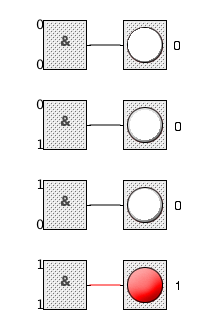
\includegraphics{figuren/boole/enpoort.png}
\caption{Een en-poort voor de vier mogelijke inputcombinaties}
\label{fig:enpoort}
\end{center}
\end{figure}
	
  \item  \textbf{Of-poort}:
Als \'{e}\'{e}n van beide, of beide ingangen op 1 gezet worden, wordt de uitgang ook 1 (figuur~\ref{fig:ofpoort}). De uitgang krijgt alleen de waarde 0 als beide ingangen 0 zijn.	

\begin{figure}[htb]
\begin{center}
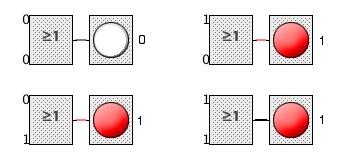
\includegraphics{figuren/boole/ofpoort.png}
\caption{Een of-poort voor de vier mogelijke inputcombinaties}
\label{fig:ofpoort}
\end{center}
\end{figure}

  \item \textbf{Niet-poort (invertor)}:
Een invertor keert de waarheidswaarde van de ingang om. (figuur~\ref{fig:nietpoort})
\end{enumerate}
%
\begin{figure}[htbp]
\begin{center}
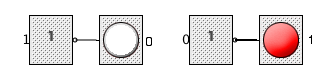
\includegraphics{figuren/boole/notpoort.png}
\caption{Een niet-poort (invertor)}
\label{fig:nietpoort}
\end{center}
\end{figure}	
 
Keren we nu terug naar het autogordel-alarm probleem. Ga na dat het circuit in figuur~\ref{fig:autoalarm} inderdaad voldoet aan de samengestelde formule voor A. Figuur~\ref{fig:autoalarm} geeft de situatie weer dat er links en rechts iemand in de zetel zit, waarbij de linkse persoon zijn gordel niet en de rechtse persoon zijn gordel wel draagt. Het contact is opgezet en de versnelling is ingeschakeld, zodat het alarm weerklinkt.

Het circuit van figuur~\ref{fig:autoalarm} is ingewikkeld. In volgende sectie over Boolse Algebra zullen we ons ondermeer bezighouden met de vraag of er een circuit mogelijk is dat eveneens voldoet aan de vereisten, maar minder poorten bevat.
%
\begin{figure}[htbp]
\begin{center}
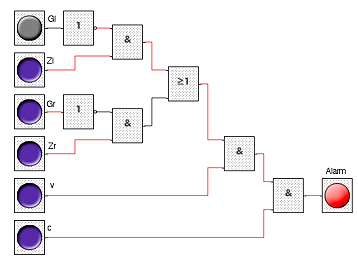
\includegraphics{figuren/boole/autoalarm.png}
\caption{Elektronische realisatie van het autogordel-alarm}
\label{fig:autoalarm}
\end{center}
\end{figure}



\newpage
\section{Boolse Algebra}
 \subsection{Definitie}
Een algebra is een verzameling elementen (zoals de verzameling van de rationale getallen) met specifieke regels voor ondermeer de optelling en de vermenigvuldiging van elementen. We introduceren het begrip `Boolse Algebra' via de 7 \emph{postulaten van Huntington}.
\begin{enumerate}
  \item Er bestaat een verzameling K van elementen, die onderworpen is aan een equivalentierelatie (genoteerd `=') die voldoet aan het substitutieprincipe.
Hiermee wordt bedoeld dat als $a = b$, $a$ in elke uitdrukking waar een $b$ in voorkomt, in de plaats van die $b$ mag gezet worden, zonder dat dit iets verandert aan de geldigheid van de uitdrukking.
  \item \begin{enumerate}
  	\item Er wordt een bewerking `+' gedefinieerd, zodanig dat $a + b$ tot K behoort, als ook $a$ en $b$ tot K behoren.
 	 \item  Er wordt een bewerking `$\cdot$' (maal) gedefinieerd, zodanig dat $a \cdot b$ tot K behoort, als ook $a$ en $b$ tot K behoren.
\end{enumerate}
  \item \begin{enumerate}
 	 \item Er bestaat een element 0 in K, zodanig dat voor elke $a$ uit K, $a + 0 = a$;
	  \item Er bestaat een element 1 in K, zodanig dat voor elke $a$ uit K, $a \cdot 1 = a$;
\end{enumerate}
  \item \begin{enumerate}
 	 \item $a + b = b + a$;
 	 \item $a \cdot b = b \cdot a$;
\end{enumerate}
  \item \begin{enumerate}
  	\item $a + (b \cdot c) = (a + b) \cdot (a + c)$;
 	 \item $a \cdot (b + c) = (a \cdot b) + (a \cdot c)$.
\end{enumerate}
  \item Voor elke element $a$ uit K bestaat er een element $\overline{a}$ (`het complement' genoemd), zodanig dat $a \cdot \overline{a} = 0$ en $a + \overline{a} = 1$.
  %%% , weggelaten voor en
  \item  K bevat minstens twee elementen $x$ en $y$, zodanig dat $x \ne y$.
\end{enumerate}

Deze postulaten vertonen nogal wat gelijkenis met die uit de gewone algebra (2: inwendigheid; 3: neutraal element; 4: commutativiteit). Ook de distributiviteit van 5 (b) herken je wel. Postulaat 5 (a) is echter totaal vreemd en gaat in tegen de regels van de `gewone' algebra. Tevens is er in de gewone algebra geen complement gedefinieerd.


\subsection{Voorbeeld 1: De verzameling $\{0,1\}$ is een Boolse algebra}
Bemerk dat in de definitie hierboven bijna niets (behalve postulaat 7) gezegd wordt over het aantal of het type van de elementen van de verzameling K. Er zijn dan ook veel structuren denkbaar die voldoen aan deze 7 postulaten. E\'{e}n van de eenvoudigste --- tevens ook diegene die ons het meest aanbelangt --- bestaat uit twee elementen, nl.\  0 en 1. De Boolse Algebra bestaande uit deze elementen wordt als volgt gedefinieerd:
%%% enkelvoud (niet worden)
\begin{displaymath}
	\overline{1}=0 \mbox{ en } \overline{0}=1
  \end{displaymath}
\begin{displaymath}
	1 \cdot 1 = 1 + 1 = 1 + 0 = 0 + 1 = 1
  \end{displaymath}
\begin{displaymath}
	0 + 0 = 0 \cdot 0 = 1 \cdot 0 = 0 \cdot 1 = 0
  \end{displaymath}
  %%% regel toegevoegd
Met  `gedefinieerd' bedoelen we dat er bepaald wordt hoe `$+$' en `$\cdot'$ werken, wat `$\overline\cdot$' is enz.
Je kan zelf eens nagaan dat deze structuur voldoet aan alle 7 postulaten.


\subsection{Voorbeeld 2: Propositielogica is een Boolse algebra}
Er is een eenduidig verband (tabel~\ref{tbl:verband}) tussen propositielogica en de eenvoudige structuur die hierboven beschreven staat. (In tabel~\ref{tbl:verband} is $p$ een willekeurige uitspraak.)
\begin{table}[htb]
  \centering
	\begin{tabular}{|c|c|}
\hline
Propositielogica & Boolse Algebra \\
\hline \hline
 $\en$  & $\cdot$  \\
 $\of$  & $+$  \\
  contradictie & 0  \\
  wet & 1 \\
  $\niet p$ & $\overline{p}$ \\
\hline
\end{tabular}
  \caption{Eenduidig verband tussen propositielogica en Boolse Algebra}\label{tbl:verband}
\end{table}

%nieuw
\subsection{Voorbeeld 3: De verzameling van alle deelverzamelingen van een universum $\Omega$ is een Boolse algebra}
\label{sec:venndiagrammen}
Nemen we als voorbeeld $\Omega=\R$ met $\R$ de verzameling van de re\"ele getallen. Noem $K$ de verzameling van alle deelverzamelingen van $\R$.\\
De bewerkingen op elementen $A$ en $B$ van $K$ (dus deelverzamelingen van $\R$) zijn als volgt gedefinieerd:
\begin{enumerate}
  \item  de doorsnede $A\cap B$  is de verzameling van alle elementen van $\R$ die tot A \emph{en} tot B behoren;
  \item de unie $A\cup B$  is de verzameling van alle elementen in $\R$ die tot A \emph{of} tot B behoren;
  \item $A^c$, het complement van $A$, is de verzameling van alle elementen in $\R $ die \emph{niet} tot A behoren.
\end{enumerate}

Deze gekende bewerkingen op verzamelingen kunnen we interpreteren als bewerkingen op elementen van een Boolse Algebra. In tabel~\ref{tbl:verbandKV} lees je het verband af. We kunnen dus stellen dat de verzameling $K$, bestaande uit alle deelverzamelingen van $\R$, een Boolse algebra is.
 % Aangezien we voor elke uitspraak $x\in A$ kunnen zeggen of ze waar(=1) of onwaar(=0) is vinden we het volgend verband, zie tabel  \ref{tbl:verbandKV} tussen logica, verzamelingenleer en Boolse Algebra.
 \begin{table}[htb]
  \centering
\begin{tabular}{|c|c|c|}
\hline
 propositielogica  & Boolse Algebra & verzamelingenleer \\ \hline \hline
  $\en$ & $\cdot$ & $\cap$ \\
   $\of$ & $+$ & $\cup$ \\
   waar & 1 & universum $\Omega$\\
   vals & 0  & $\emptyset$ \\
   $\niet a$ & $\overline{a}$ & $A^c$ \\
\hline
\end{tabular}
  \caption{Verband tussen Boolse algebra, propositielogica en verzamelingenleer}\label{tbl:verbandKV}
\end{table}

\subsubsection{Postulaten}
We controleren of de verzameling $K$ met de in tabel~\ref{tbl:verbandKV} gedefinieerde kenmerken voldoet aan de postulaten van Huntington:

Voor alle deelverzamelingen $A$ en $B$ en $C$ van $\R$ geldt
\begin{enumerate}
\item $A \cup B \in K$ (de unie van twee deelverzamelingen is steeds een nieuwe deelverzameling);
\item $A \cap B \in K$ (\dots);
\item $A \cup \emptyset = A$ (postulaat \dots);
\item $A \cap \Omega= A$ (\dots);
\item $A \cap B = B \cap A$;
\item $A \cup B = B \cup A$;
\item $A \cup A^c=\Omega$ (\dots);
\item $A \cap A^c=\emptyset$ (\dots).
\item $ A \cap (B \cup C)= (A \cap B) \cup (A \cap C)$;
\item $ A \cup (B \cap C)= (A \cup B) \cap (A \cup C)$;
\end{enumerate}


\subsubsection{Eigenschappen}
Je kan ook een aantal eigenschappen afleiden voor  de verzameling $K$. Controleer deze eigenschappen met Venndiagrammen. Deze voorstelling van verzamelingen heeft bewijskracht.

Voor alle deelverzamelingen $A$ en $B$ van $\R$ geldt
\begin{enumerate}
\item $A \cap \emptyset = \emptyset$;
\item $A \cup \Omega= \Omega$;
\item $(A \cup B)^c=A^c \cap B^c$;
\item $(A \cap B)^c=A^c \cup B^c$;
\item $A \cap A=A$;
\item $A\cup A=A$.
\item $(A^c)^c=A$
\end{enumerate}
% moet nog worden aangepast
%\begin{figure}[htbp]
%\begin{center}
%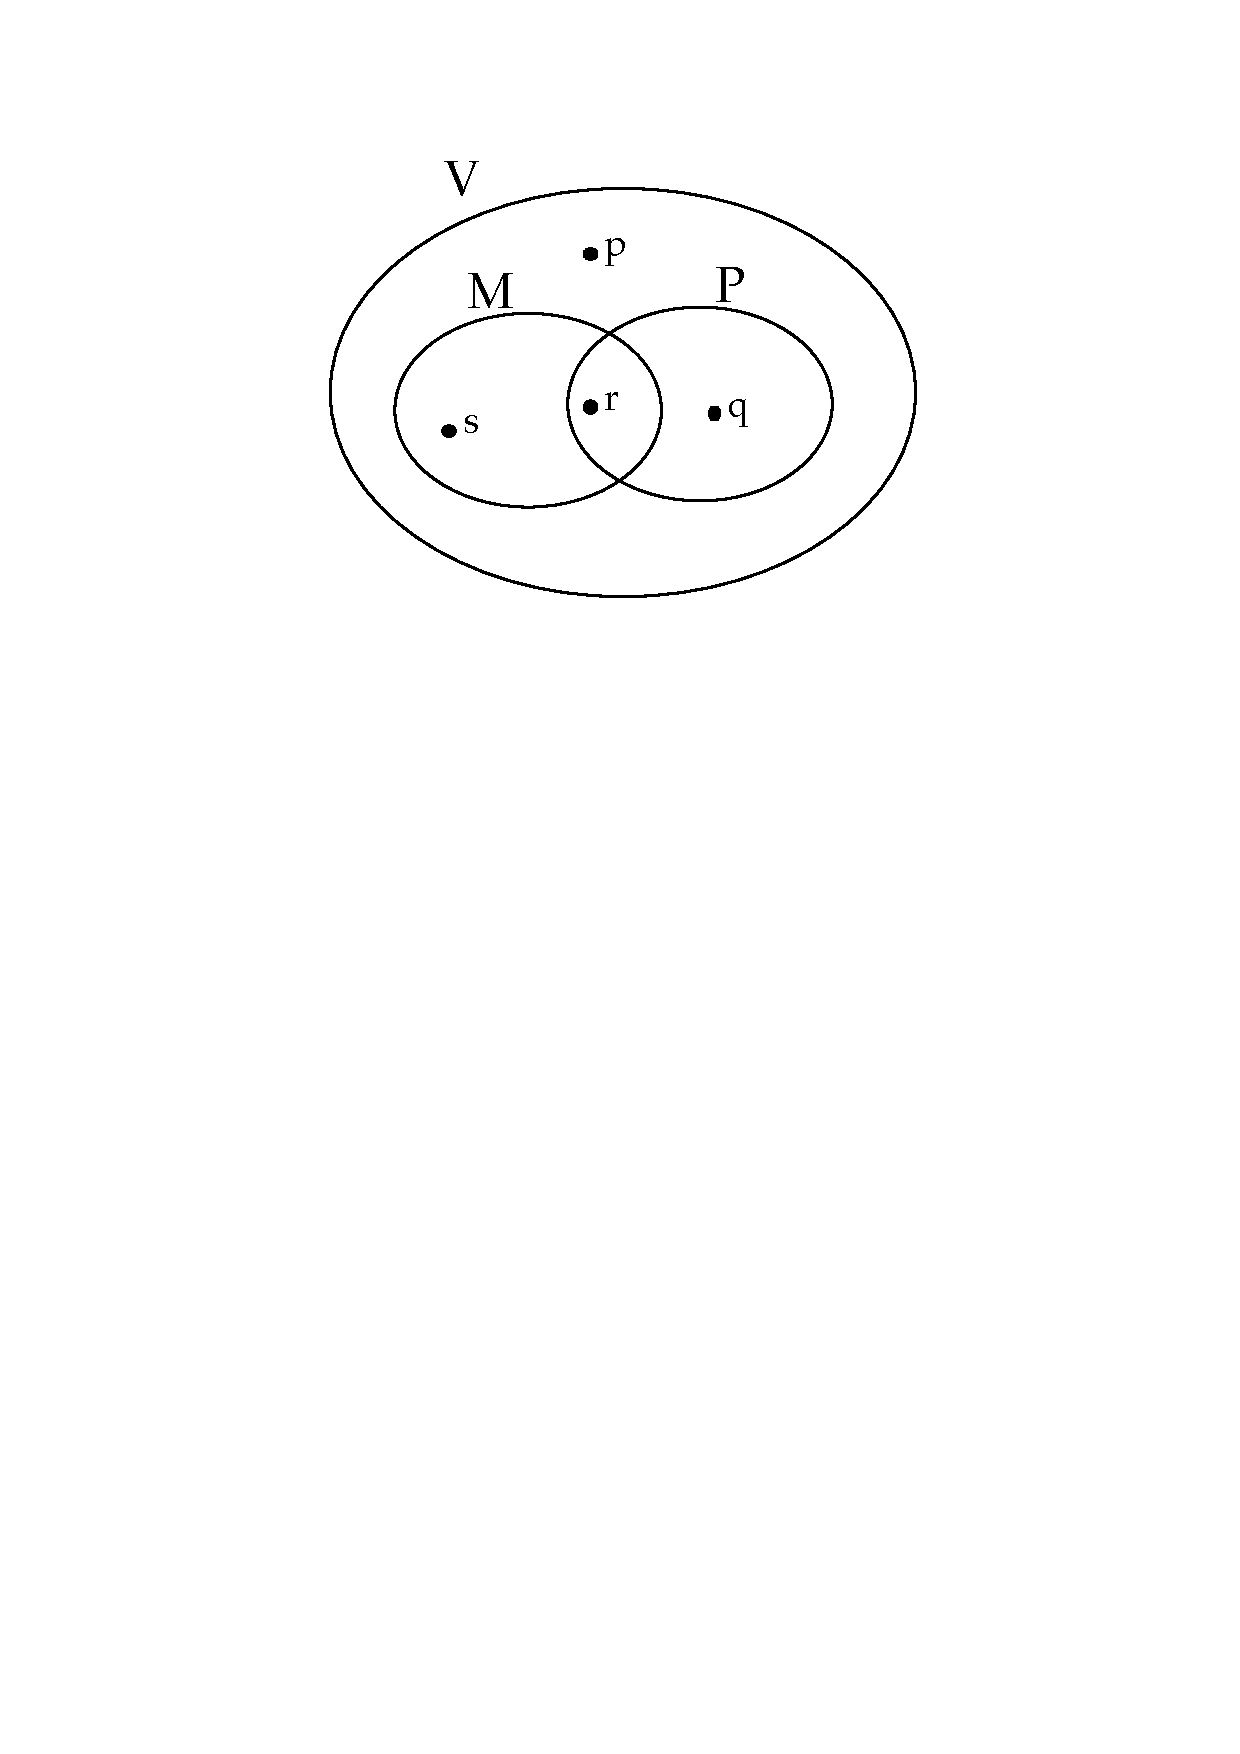
\includegraphics[bb= 100 550 500 800,clip,width=\textwidth]{figuren/boole/venndiagram.pdf}
%\caption{Venn-diagram}
%\label{fig:venn}
%\end{center}
%\end{figure}


\subsection{Dualiteit}
Vier van de zeven postulaten van Huntington komen voor in paren. Als je nauwkeurig toekijkt, merk je dat je telkens \'{e}\'{e}n van de twee kan bekomen door in het tweede postulaat elke `+' te vervangen door `$\cdot$', en elke `0' door `1' (en omgekeerd).
Dit \emph{dualiteitsprincipe} kan toegepast worden voor elke stelling of eigenschap die we nog zullen zien (`twee stellingen voor de prijs van \'{e}\'{e}n!', zie bijvoorbeeld tabel~\ref{tbl:eig}). Deze eigenschap van dualiteit zullen we gebruiken om een tweede standaardvorm van Boolse veeltermen te bepalen (zie sectie~\ref{sec:standaardvorm}), alsook om een tweede algoritme te vinden voor het minimaliseren van Boolse functies (sectie~\ref{sec:minimalisatie}).

In deze nota's vind je alleen de uitleg voor de \emph{eerste standaardvorm}. Je zoekt zelf via dualiteit \emph{de definities en het algoritme} voor de tweede. Op het einde van dit hoofdstuk vind je een \emph{onvolledig} overzicht van de belangrijkste algoritmen voor de eerste standaardvorm. Nadat je dit overzicht aangevuld hebt kan je het gebruiken om zelf de duale vormen op te stellen.  Daarna test je die tweede standaardvorm uit op een concreet voorbeeld. In de oefeningen kan je bijkomende uitleg vragen.

Regelmatig wordt in de tekst de formulering van de duale standaardvorm tussen vierkante haakjes vermeld.

\subsection{Eigenschappen in een Boolse Algebra}
De postulaten van Huntington geven aanleiding tot een aantal eigenschappen van een Boolse Algebra. Het verschil tussen een postulaat en eigenschap is het volgende: een postulaat wordt \emph{gedefinieerd} (iemand zegt dat het zo moet zijn), een eigenschap volgt uit de postulaten (kan je bewijzen). In sectie~\ref{sec:venndiagrammen} heb je een aantal eigenschappen van de verzameling $K$ bestaande uit alle deelverzamelingen van $\R$ reeds bewezen.

Tabel~\ref{tbl:eig} vermeldt de meest gebruikte of de eenvoudigste eigenschappen. Kan je de eigenschappen van sectie~\ref{sec:venndiagrammen} herkennen? Welke eigenschappen ontbreken in het overzicht van die sectie?

Omwille van de dualiteit (zie bovenstaande sectie) zetten we de duale eigenschappen naast elkaar in twee kolommen. De voornaamste bedoeling is de kracht van het principe van dualiteit te illustreren.
\begin{table}
  \centering
\begin{tabular}{|c|c|c|}
\hline
 Naam  & Optelling & Vermenigvuldiging \\
\hline \hline
 opslorpende eigenschap  & $x+1=1$ & $x \cdot 0 = 0$ \\
 idempotentie  & $x+x=x$ & $x \cdot x = x$ \\
 associativiteit & $x+(y+z)=(x+y)+z$ & $x \cdot (y \cdot z)=(x \cdot y) \cdot z$ \\
 involutiviteit van compl. & \multicolumn{2}{c|}{$\overline{\overline{x}}=x$} \\
 wetten van de Morgan & $\overline{x+y}=\overline{x} \cdot \overline{y}$ & $\overline{x \cdot y}=\overline{x}+\overline{y}$ \\
 absorptiewet & $x+(x \cdot y)=x$ & $x \cdot (x+y)=x$ \\
\hline
\end{tabular}
  \caption{Enkele eigenschappen en hun duale}\label{tbl:eig}
\end{table}

Laten we een voorbeeld bekijken van de nauwe band tussen propositielogica en Boolse Algebra, met name de `involutiviteit van het complement' uit tabel~\ref{tbl:eig}: $\overline{\overline{x}}=x$. In Boolse Algebra lees je deze wet als ``Het complement van het complement van een veranderlijke is de veranderlijke zelf''. In het taalgebruik van propositielogica klinkt dit als ``De negatie van de negatie van een uitspraak is de uitspraak zelf''. Met een voorbeeld: als we zeggen dat het \emph{niet waar} is dat het \emph{niet} regent dan bedoelen we dat het regent. Bij verzamelingenleer kan dat klinken als ``alle elementen die tot $\Omega$ behoren en niet tot $A^c$,  zitten in A. Alle elementen van A behoren ook niet tot $A^c$.''

\subsection{Boolse Veelterm -- tweewaardige Boolse functie}
\subsubsection{Definities}\label{subsec:def}
Een \emph{Boolse veelterm} is elke uitdrukking in een aantal veranderlijken (gewoonlijk nemen we $x$, $y$, $z$ of $a$, $b$, $c$,...) met de bewerkingen `$+$', `$\cdot$' en het complement, en de speciale elementen 0 en 1. De bewerking `$\cdot$' heeft voorrang op de `$+$' (net zoals in propositielogica de bewerking  `en' voorrang heeft op `of').\\

\noindent
Een \emph{tweewaardige Boolse functie} kunnen we beschouwen als een `black box', waar de Boolse veranderlijken dienst doen als input, en waar er \'{e}\'{e}n output is die slechts twee waarden (vandaar \emph{twee}waardig) kan krijgen: 0 en 1.
Zo'n functie komt dus in principe overeen met een \emph{waarheidstabel} die voor elke input de output weergeeft (zonder te laten zien hoe men aan die output komt). Als synoniem gebruiken we soms de term `schakelfunctie'.
% Een tweewaardige Boolse functie zullen we vanaf nu meestal met de benaming `\emph{schakelfunctie}' aanduiden. De veranderlijken die als input voor zo'n functie dienen noemen we `\emph{schakelvariabelen}'.

\subsubsection{Bij elke Boolse veelterm hoort een tweewaardige Boolse functie}

Beschouw de Boolse veelterm  $x + (y + y\cdot z)$. Dit is inderdaad een uitdrukking in de drie Boolse veranderlijken $x$, $y$ en $z$ die aan de definitie van sectie~\ref{subsec:def} voldoet. Aan deze \emph{veelterm} kunnen we de Boolse \emph{functie}
\begin{displaymath}
f(x, y, z) = x + (y + y\cdot z)
\end{displaymath}
verbinden. In wat volgt laten we zien hoe de veelterm $x + (y + y\cdot z)$ aanleiding geeft tot de `black box' voorstelling van de functie $f(x,y,z)$.

Voor de Boolse functie $f(x,y,z)$ kan er een lijst opgemaakt worden van alle mogelijke inputs en corresponderende output met behulp van de verbonden veelterm $x + (y + y\cdot z)$. Bijvoorbeeld, geven we aan de Boolse veranderlijken de input $x=0$, $y=1$ en $z=1$, dan vinden we (via berekeningen) als output voor de veelterm $0+(1+1\cdot 1)=0+1=1$. Er zijn 8 verschillende inputs: elke input kan 2 waarden aannemen zodat er $2\cdot 2 \cdot 2=2^3=8$ mogelijkheden zijn. Deze lijst (8 inputs met bijhorende output) bepaalt de Boolse functie $f(x,y,z)$ volledig.  Daarom zeggen we dat bij elke  Boolse veelterm een tweewaardige Boolse functie hoort.
\begin{figure}[htbp]
\begin{center}
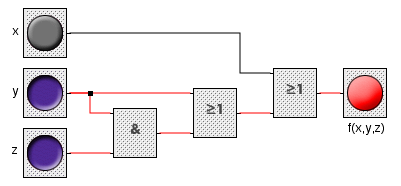
\includegraphics[width=\textwidth]{figuren/boole/voorbeeld.png}
\caption{Realisatie van $x+(y+yz)$}
\label{fig:schakelvb}
\end{center}
\end{figure}



Bovenvermelde lijst vormt bovendien de \emph{waarheidstabel} van de Boolse functie $f(x,y,z)$. Je vindt ze in tabel~\ref{tbl:schakelvb}. Omdat de waarheidstabel \emph{zonder dat de verbonden veelterm gekend hoeft te zijn} iedere mogelijke input van de functie verbindt met  de corresponderende output, spreekt men van een `black box'.

\begin{table}
  \centering
  \begin{tabular}{|ccc|c|}
\hline
  $x$ & $y$ & $z$ & $f(x,y,z)$ \\ \hline \hline
 0  & 0 & 0 & 0 \\
 0  & 0 & 1 & 0 \\
 0  & 1 & 0 & 1 \\
 0  & 1 & 1 & 1 \\
 1  & 0 & 0 & 1 \\
 1  & 0 & 1 & 1 \\
 1  & 1 & 0 & 1 \\
 1  & 1 & 1 & 1 \\
\hline
\end{tabular}
  \caption{Waarheidstabel horend bij $f(x,y,z)=x+(y+yz)$}\label{tbl:schakelvb}.
\end{table}


Van de veelterm kunnen we de \emph{fysische realisatie} tekenen. Elke bewerking komt overeen met een poort. Ga zelf na dat onderstaand schema (figuur~\ref{fig:schakelvb}) de fysische realisatie met elektronische poorten is van deze functie. Als je het circuit simuleert, merk je dat je de waarden van de waarheidstabel bekomt. Als je bijvoorbeeld als input de vierde rij uit de waarheidstabel geeft, vind je 1 als output.

\subsubsection{Samenvatting}
\begin{itemize}
\item Noem $V$ de verzameling van alle Boolse veeltermen in 3 veranderlijken. Hoeveel zijn er denk je?
\item Noem $W$ de verzameling van alle waarheidstabellen in 3 Boolse veranderlijken. Hoeveel kan je er noteren?
\item Noem $F$ de verzameling van alle fysische realisaties met 3 input veranderlijken.
\end{itemize}
Als je de drie verzamelingen tekent, kan je een pijl trekken van $V$ naar $F$ en omgekeerd: de bewerkingen kan je altijd door juist \'e\'en poort vervangen en omgekeerd. We hebben hierboven verantwoord dat er een \'e\'enduidige relatie is van de verzameling $V$ naar $W$ (trek een pijl van $V$ naar $W$): bij iedere Boolse veelterm hoort juist \'e\'en Boolse functie (`black box', waarheidstabel). Verder in de tekst (zie \ref{subsec.pijl}) leggen we een relatie van  $W$  naar $V$.
\label{pag:VnaarW}



%\subsubsection{Veralgemeende poorten}
%Elektronisch is het mogelijk om ook `en'- en `of'-poorten te maken met meer dan twee ingangen. Deze \emph{veralgemeende poorten} zullen we verderop nodig hebben. Figuur~\ref{fig:alg_enpoort} toont en-poorten met drie en vier ingangen. Ze zijn in LogicSim eenvoudig aan te maken. Alles wat je moet doen, is eerst onderaan links het aantal ingangen kiezen (van 2 tot 5), en vervolgens de gewenste poort kiezen (en, of).
%\begin{figure}[htbp]
%\begin{center}
%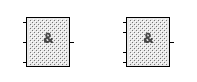
\includegraphics{figuren/boole/algemene_enpoort.png}
%\caption{en-poorten met drie en vier ingangen}
%\label{fig:alg_enpoort}
%\end{center}
%\end{figure}


\newpage
\section{Minimalisatie van Boolse functies}
\label{sec:minimalisatie}
\subsection{Inleiding}
We kunnen ons nu de vraag stellen of we bvb.\ de functie  
\begin{displaymath}
f(x,y,z)=x+(y+yz)
\end{displaymath}
 niet op een voordeliger manier kunnen noteren (d.w.z.\ met minder Boolse bewerkingen) waarbij het gedrag (= de functiewaarden) voor alle 8 rijen uit de tabel hetzelfde blijven. We zeggen dat de nieuwe veelterm gelijkwaardig moet zijn aan de originele.

\subsubsection{Definitie}
\noindent
Twee Boolse veeltermen zijn \emph{gelijkwaardig} als ze dezelfde Boolse functie (=waarheidstabel) genereren.\\

Wie naar tabel~\ref{tbl:schakelvb} kijkt, merkt bvb.\ op dat de waarde van $z$ blijkbaar geen rol speelt. Test dit ook uit via een simulatie. We verwachten dus een gelijkwaardige schakeling waarin $z$ niet meer hoeft verbonden te worden  met een poort.  Met hulp van de postulaten en eigenschappen van Boolse algebra berekenen we:
\begin{eqnarray*}
f(x,y,z) & = & x + (y + y\cdot z) \\
 & = & x + y(1 + z) \mbox{ \hspace{1cm}  (distributiviteit)} \\
 & = & x + y	\mbox{ \hspace{1cm}   (1 + $z$ = 1, onafhankelijk van $z$)}
\end{eqnarray*}
Blijkbaar kan de Boolse veelterm $f$ ook gerealiseerd worden zoals op figuur~\ref{fig:eenvoudiger}.

We hebben bij wijze van `smaakmaker' dit voorbeeld uitgewerkt via rekenwerk in een Boolse algebra. Dit is echter niet altijd mogelijk. In een volgende sectie van dit hoofdstuk zullen we deze vereenvoudiging systematisch aanpakken.
\begin{figure}[htbp]
\begin{center}
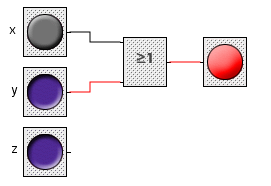
\includegraphics{figuren/boole/eenvoudigervb.png}
\caption{Eenvoudiger circuit}
\label{fig:eenvoudiger}
\end{center}
\end{figure}



\subsection{Standaardvormen van Boolse functies} \label{subsec.pijl}
\label{sec:standaardvorm}
In de vorige sectie vereenvoudigden we een functie via algebra\"{i}sch rekenwerk. Dit lukte omdat het ging om een eenvoudig voorbeeld. We hebben echter nOPO aan een meer systematische manier om Boolse functies te vereenvoudigen.

Hiervoor gebruiken we een van de twee \emph{standaardvormen}. In wat volgt ontwikkelen we slechts \'e\'en ervan. [De tweede standaardvorm kan bekomen worden door dualiteit, opdracht voor de student]. Gelijkwaardige Boolse functies kunnen steeds tot dezelfde standaardvorm herschreven worden. Het spreekt voor zich dat deze standaardvorm ook gelijkwaardig is aan de gegeven functies. De standaardvorm is dus als het ware een prototype voor een verzameling gelijkwaardige functies.

We beginnen met de definitie van een aantal begrippen.
\subsubsection{Definities}

\noindent
Een \emph{productterm} [somterm] is een opeenvolging van variabelen (of het complement ervan) verbonden door een vermenigvuldiging (`en' = `$\cdot$' die vaak niet meer geschreven wordt), bvb.\ $ac$ (in plaats van $a \cdot c$), $a\overline{b}d$. Merk op dat $\overline{ac}d$ geen productterm is (leg uit waarom).\\

\noindent
Als elke variabele in een productterm hoogstens \'{e}\'{e}n keer voorkomt (dus juist \'e\'en keer of niet), noemen we de term een \emph{normale productterm}  of \emph{normaalvorm}. De normaalvorm kan je beschouwen als de meest `effici\"{e}nte' vorm van de productterm, vermits een herhaald voorkomen van een variabele ofwel overbodig is  ($a \cdot a = a$), ofwel aanleiding geeft tot een triviale functie ($a \cdot \overline{a} = 0$).\\

\noindent
Als in een normale productterm elke variabele van de functie \emph{juist \'e\'en keer} voorkomt dan noemen dit een \emph{standaard productterm}, kortweg een \emph{minterm} [maxfactor]. \\

\noindent
Een Boolse veelterm die uitsluitend bestaat uit de som van standaard producttermen is een \emph{standaard som van producten}.


\subsubsection{Een Boolse veelterm omzetten naar een standaard som van producten}
We bekijken twee voorbeelden, waarin we een 2-waardige Boolse functie herschrijven tot een standaard som van producten. Vervolgens leiden we hieruit de algemene werkwijze af.
\begin{enumerate}
  \item \textbf{Voorbeeld}: Herwerk de functie $f(a,b,c,d)=(ac+b)(cd+\overline{d})$ tot een standaard som van producten \\
\textbf{Oplossing}:
De opgave is een product van sommen waarin nog producten voorkomen.
\begin{eqnarray*}
f(a,b,c,d) & = & (ac+b)(cd+\overline{d}) \\
 & = & (ac+b)cd+(ac+b)\overline{d} \mbox{\hspace{1cm}(distributiviteit)} \\
 & = & accd+bcd+ac\overline{d}+b\overline{d}  \mbox{\hspace{1cm}(distributiviteit)} \\
 & = & acd+bcd+ac\overline{d}+b\overline{d}  \mbox{\hspace{1cm}(vereenvoudiging: } cc=c \mbox{ )}
\end{eqnarray*}

We bekomen nu een som van (normale) producten, waarbij in elke normale term minstens \'e\'en veranderlijke ontbreekt. Om die producttermen te vervolledigen tot een minterm (waar iedere variabele juist \'e\'en keer moet voorkomen) maken we gebruik van de eigenschappen  $a + \overline{a} = 1$ en dat $a \cdot 1 = a$. We passen dit in voorgaande som toe enkel voor de eerste en de laatste term. Je kan zelf de tussenliggende termen vervolledigen.
\begin{eqnarray*}
f(a,b,c,d) & =  & acd+\ldots+b\overline{d} \\
 & =  & acd \cdot 1+\ldots+b\overline{d}\cdot 1 \\
 & = &acd(b+\overline{b})+\ldots+bd(a+\overline{a}) \\
 & = & abcd+a\overline{b}cd+\ldots+ab\overline{d}+\overline{a}b\overline{d} \\
 & = & abcd+a\overline{b}cd+\ldots+ab\overline{d}(c+\overline{c})+\overline{a}b\overline{d}(c+\overline{c}) \\
 & = & abcd+a\overline{b}cd+\ldots+abc\overline{d}+ab\overline{c}\overline{d}+\overline{a}bc\overline{d}+\overline{a}b\overline{c}\overline{d}
\end{eqnarray*}

Vergeet niet na het uitwerken van alle vervolledigingen de gelijke mintermen te schrappen want $x+x=x$.
De hele som is de gevraagde \emph{standaard som van producten}, ook wel \emph{som van mintermen} genoemd.


  \item \textbf{Voorbeeld}: Herwerk de functie $f(a,b,c,d,e)=(\overline{ac}+\overline{d})(\overline{b+ce})$ tot een som van producten \\
\textbf{Oplossing}:
\begin{eqnarray*}
f(a,b,c,d,e) & = &  (\overline{ac}+\overline{d})(\overline{b+ce})\\
 & = & ((\overline{a}+\overline{c})+\overline{d})(\overline{b} \cdot \overline{ce})) \\
 & = & ((\overline{a}+\overline{c})\overline{b}+\overline{d}\cdot b)(\overline{c}+ \overline{e}) \\
 & = & (\overline{a}\cdot \overline{b}+\overline{b}\cdot \overline{c}+\overline{b}\cdot \overline{d})(\overline{c}+ \overline{e}) \\
 & = & \overline{a}\cdot \overline{b}\cdot \overline{c}+\overline{b}\cdot \overline{c}+\overline{b}\cdot \overline{c}\cdot \overline{d}+\overline{a}\cdot \overline{b}\cdot \overline{e}+\overline{b}\cdot \overline{c}\cdot \overline{e}+\overline{b}\cdot \overline{d}\cdot \overline{e}
\end{eqnarray*}
\end{enumerate}
Vervolledig zelf de tweede en de laatste term totdat je een som van mintermen bekomt in 5 veranderlijken.

%In bovenstaand voorbeeld herken je twee keer een toepassing van de wet van De Morgan, en twee keer een toepassing van de distributiviteit. Merk ook op dat we gewoonlijk de letters in alfabetische volgorde zetten waar dat kan (toepassing van de commutativiteit). Dit resultaat is nog geen unieke voorstelling van de veelterm.
	
%Bekijken we nog eens de einduitkomst van het eerste voorbeeld. Het is mogelijk om deze vorm te herwerken tot er uiteindelijk een som van producten staat, waarbij elk product de 4 variabelen (of het complement) moet bevatten.
% (en natuurlijk ook van de distributiviteit). Om het geheel niet nodeloos te verzwaren wordt alleen de eerste en de laatste term van voorbeeld 1 overgeschreven. Probeer zelf eens de volledige uitwerking te maken.


Uit deze twee voorbeelden leiden we \emph{het algoritme} af om elke Boolse veelterm via rekenen in een Boolse Algebra om te zetten naar een \emph{standaard som van producten}.
\subsubsection{Algoritme}
\begin{enumerate}
  \item Werk alle complementen uit die boven een bewerking `$+$' of  '$\cdot$' staan via de \emph{wetten van De Morgan}.
  \item Pas de \emph{distributiviteit} toe ( `$\cdot$' ten opzichte van `$+$') zodat je een som van producten bekomt. Je doet dit eventueel meerdere keren na elkaar.
	\item \emph{Vereenvoudig} tussenin, zie eigenschappen van de Boolse Algebra.
	\item \emph{Vervolledig} elke normale productterm tot een standaard productterm (minterm).
	\item  Vereenvoudig.
\end{enumerate}

\noindent
Volgende \textbf{stelling} geldt:
\begin{quote}
 Elke 2-waardige Boolse functie $f(x_{1}, x_{2},\ldots ,x_{n})$ van $n$ veranderlijken kan als een standaard som van producten geschreven worden. (Stelling~1)
\end{quote}
\label{pag:stelling1}

\noindent
De aandachtige lezer zal terecht opmerken dat er van \emph{vereenvoudiging} niet echt sprake is. De uiteindelijke standaardvorm is veel ingewikkelder dan de uitdrukking waarvan we vertrokken. Hij is echter wel uniek, en vormt aldus een goed \emph{vertrekpunt voor het vereenvoudigingsalgoritme}.

\subsubsection{Terminologie voor de duale standaardvorm}
somfactor; normaalfactor; standaard somfactor = maxfactor; standaard product van sommen = een product van maxfactoren.

%Het is de taak van de student het algoritme voor de duale vorm  \textbf{standaard product van sommen (Maxfactoren)} op te stellen. In de oefeningen worden er hierop toepassingen gemaakt.
\subsubsection{Opdrachten}
\begin{enumerate}
  \item Hoeveel mintermen in 3 veranderlijken kan je vormen? Verklaar.
  \item Hoeveel verschillende standaard sommen van producten kan je neerschrijven?
  \item Waarom kies je hier in het algoritme voor de eigenschap van distributiviteit van `$\cdot$' t.o.v.\ van `$+$'?
\end{enumerate}

\subsection{Functies beschrijven d.m.v. mintermen}
Bovenstaand verhaal leverde een manier op om elke Boolse veelterm om te vormen tot een \emph{standaard som van producten} of som van mintermen.
In wat volgt gaan we  op \'e\'enduidige manier een standaard som van producten associ\"eren aan een tweewaardige Boolse functie (=waarheidstabel). We leggen dus de relatie van $W$ naar $V$ (zie pag.~\pageref{pag:VnaarW}).

\subsubsection{Korte notatie voor waarheidstabel}
We zoeken eerst een \emph{korte notatie} voor de waarheidstabel die bij een tweewaardige Boolse functie $f(a,b,c)$ hoort. We veronderstellen dat we de veelterm (functievoorschrift) niet kennen.

We nummeren de rijen van de waarheidstabel en schrijven alleen die nummers op waarvoor de functie output 1 heeft. Deze informatie legt de \emph{volledige} waarheidstabel vast aangezien er slechts twee waarden (0 en 1) zijn voor de output.

We werken dit uit voor een voorbeeld. Tabel~\ref{tbl:onbekfunctie} toont de waarheidstabel van een functie $f(a,b,c)$.
\begin{table}[htb]
  \centering
 \begin{tabular}{|ccc|c|}
\hline
$a$  & $b$ & $c$ & $f$ \\ \hline \hline
  0 & 0 & 0 & 1 \\
  0 & 0 & 1 & 0 \\
  0 & 1 & 0 & 0 \\
  0 & 1 & 1 & 0 \\
  1 & 0 & 0 & 1 \\
  1 & 0 & 1 & 1 \\
  1 & 1 & 0 & 0 \\
  1 & 1 & 1 & 1 \\
\hline
\end{tabular}
  \caption{Een functie gegeven door haar waarheidstabel}\label{tbl:onbekfunctie}
\end{table}
We bekijken elke inputcombinatie voor  $a,b,c$  als een binair getal. Zo bvb.\ staat op de vierde rij in de tabel $a = 0$, $b = 1$ en $c = 1$. Het binair getal $011$ komt overeen met het getal 3 in het decimaal stelsel. Bijgevolg geven we de vierde rij het nummer 3.
Elk rijnummer bepaalt dus \'e\'enduidig de inputwaarden van de Boolse veranderlijken. In tabel~\ref{tbl:metrijnr} voegen we de rijnummers expliciet toe.
\begin{table}[htb]
  \centering
 \begin{tabular}{|c|ccc|c|}
\hline
Rijnummer & $a$  & $b$ & $c$ & $f$ \\ \hline \hline
 0 & 0 & 0 & 0 & 1 \\
  1 & 0 & 0 & 1 & 0 \\
 2 & 0 & 1 & 0 & 0 \\
 3 & 0 & 1 & 1 & 0 \\
 4 & 1 & 0 & 0 & 1 \\
 5 & 1 & 0 & 1 & 1 \\
 6 & 1 & 1 & 0 & 0 \\
 7 & 1 & 1 & 1 & 1 \\
\hline
\end{tabular}
  \caption{De waarheidstabel met toevoeging van het rijnummer}\label{tbl:metrijnr}
\end{table}

We kunnen nu de functie $f$ \emph{noteren} door op te schrijven op welke rijen van de waarheidstabel ze output 1 heeft. We doen dit als volgt: 
\begin{displaymath}
f(a,b,c) = \sum m(0, 4, 5, 7)
\end{displaymath}
Deze notatie $\sum m  \dots $ wordt verderop verklaard. [Duaal: omschrijf de functie door aan te geven op welke rijen een 0 staat: $f(a,b,c) = \prod M(1, 2, 3, 6)$.] Deze korte notatie gaan we gebruiken om de som van mintermen (standaard som van producten) te vinden die hoort bij de gegeven waarheidstabel.

%Bekijk volgende standaard som van producten:
%\begin{displaymath}
%f(a,b,c)=\overline{a}\overline{b}\overline{c}+a\overline{b}\overline{c}+a\overline{b}c+abc
% \end{displaymath}

\subsubsection{Bijhorende standaard som van producten, mintermen}
We zoeken naar een \emph{standaard som van producten} die tabel~\ref{tbl:onbekfunctie} genereert. Uitgangspunt is Stelling~1 van blz.~\pageref{pag:stelling1}. Aangezien er 3 veranderlijken zijn, kan de som hoogstens uit 8 mintermen bestaan. Vraag is: welke van de acht?
\begin{enumerate}
  \item  Uit $a + 1 = 1$ leren we dat een som 1 wordt als  \'e\'en (of meer) van de termen gelijk aan 1 is (zijn). Concreet: omdat de output 1 is op de vierde rij bij input $a=1$, $b=0$, $c=0$ moet \'e\'en van de 8 mintermen bij die input als waarde 1 hebben.
  \item Welke van de 8 mogelijke mintermen heeft output 1 bij input 100? We weten dat een product slechts \'e\'enmaal de output 1 geeft, nl.\  als alle veranderlijken de waarde 1 hebben. Een 0 in een product geeft altijd als resultaat 0. Aangezien de input 100 is moeten we van de input-waarden die 0 zijn een 1 maken via het complementeren van de bijhorende veranderlijke. De minterm die we zoeken voor de vierde rij is dus $a\overline{b}\overline{c}$.  \emph{Reken na} dat alle andere mintermen bij input 100, output gelijk aan 0 hebben.
  \item We vinden dus een \'e\'enduidig verband tussen de minterm $a\overline{b}\overline{c}$ en de output 1 op rij nummer 4 in de waarheidstabel.  (\emph{De uniciteit is ook de reden waarom we bij output 1  een productterm associ\"eren!)} We zeggen dat deze minterm output 1 \emph{produceert} op rij $4$. We noemen de minterm $a\overline{b}\overline{c}$  \emph{minterm 4}, notatie $m_{4}$.
  \item  $m_{4}$ moet dus zeker voorkomen in \emph{de standaard som van producten} die behoort bij deze waarheidstabel. Indien we deze redenering herhalen voor elke output 1 dan vinden we  vier mintermen in \emph{de standaardsom van producten} die we zoeken.
  \item Herhaal  de redenering voor de output 1 op rij 0, 5 en 7, m.a.w zoek  $m_{0}$, $m_{5}$ en $m_{7}$. De standaardsom van producten is dan \\
  $ \overline a\overline{b}\overline{c} +a\overline{b}\overline{c} +a\overline{b} c +abc$.
  \end{enumerate}

\subsubsection{Opdrachten}
\begin{itemize}
\item Waarom mag bvb.\ de minterm $\overline{a}\cdot b\cdot \overline{c}$ niet voorkomen in deze 2-waardige Boolse functie?
  \item Stel zelf een algoritme op om de mintermen van de standaardsom van producten op te stellen uitgaande van de waarheidstabel.

  \item Wat weet je als de minterm $\overline{a}bc$ niet voorkomt in de standaardsom van producten?
  \item Geef de standaardsom van producten voor een waarheidstabel met allemaal nullen.
\end{itemize}
\subsubsection{Samenvatting}
Bij elke rij in de waarheidstabel hoort juist \'e\'en minterm, nl.\ die minterm die output 1 geeft bij de input-waarden van die rij [Zet dit zelf duaal om].
Tabel~\ref{tbl:minmax} toont enkele mintermen en maxfactoren die bij elke rij van een waarheidstabel met 3 veranderlijken horen (vul de rijen 3 t.e.m. 6 zelf aan). De uitbreiding naar meer variabelen ligt voor de hand. Voor de mintermen komt elke niet-gecomplementeerde variabele overeen met een  input 1 want de output moet 1 zijn.
\begin{table}[htb]
  \centering
 \begin{tabular}{|c|ccc|c|c|}
\hline
 rijnr.  & a & b & c & Minterm & Maxfactor \\ \hline \hline
  0 & 0 & 0 & 0  & $\overline{a}\overline{b}\overline{c}=m_{0}$ &  \\
  1 & 0 & 0 & 1  & $\overline{a}\overline{b}c=m_{1}$ & $a+b+\overline{c}=M_{1}$ \\
  2 & 0 & 1 & 0  & $\overline{a}b\overline{c}=m_{2}$ &  \\
\ldots & \ldots & \ldots & \ldots & \ldots & \ldots \\
  7 & 1 & 1 & 1  & $abc=m_{7}$ & $\overline{a}+\overline{b}+\overline{c}=M_{7}$ \\
\hline
\end{tabular}
  \caption{Mintermen en (duaal:maxfactoren) behorende bij 3 veranderlijken}\label{tbl:minmax}
\end{table}

Aangezien de waarheidstabel een 2-waardige Boolse functie volledig bepaalt en we hierboven een manier hebben ontwikkeld om elke waarheidstabel om te vormen tot een standaard som van producten, hebben we de relatie van $W$ naar $V$ gelegd (pag.~\pageref{pag:VnaarW}).  Zoals een Boolse veelterm een Boolse functie bepaalt, bepaalt een Boolse functie ook een Boolse veelterm.

Hiermee hebben we ook een manier gevonden om vanuit een waarheidstabel een elektronische schakeling te maken, immers de standaardveelterm geeft ons bewerkingen die we kunnen omzetten naar elektronische  poorten.\\
 \emph{In de praktijk is deze omzetting heel belangrijk omdat de meeste Boolse problemen vertrekken van een waarheidstabel en als doel hebben om een elektronische schakeling op te stellen.}

\subsection{Oefeningen}
\subsubsection{Oefening 1}
Vorm volgende functie om naar de $\sum m(\ldots)$ notatie:
\begin{displaymath}
\begin{array}{cccccccccc}
     f(a,b,c,d) & = & abcd & + & abc\overline{d} & + & \overline{a}bc\overline{d} & + & \overline{a}b\overline{c}d  &  \\
      &  = & 1111 & & 1110 & & 0110 & & 0101 & \mbox{(bin. input)}\\
      & = & 15 & & 14 & & 6 & & 5 & \mbox{(dec.input)}
\end{array}
  \end{displaymath}
Hieruit kunnen we besluiten: $f(a,b,c,d) = \sum m(5, 6, 14, 15)$

\subsubsection{Oefening 2}
Schrijf de \emph{standaard som van producten} op voor volgende $\sum m(\ldots)$ \\
$f(a,b,c,d)=\sum m(3,5,9,11,14)$\\

Vul de oplossing verder aan:\\
Oplossing:
\begin{displaymath}
\begin{array}{cccccccccccc}
     f(a,b,c,d) & = & 3 & + & 5 & + & 9 & + & 11 & + & 14  & \mbox{(dec. input)} \\
      &  = & 0011 & & 0101 & & 1001 & & \dots  & &\dots & \mbox{(bin. input)}\\
      & = & \overline a \overline b cd & + &\overline a b \overline c d & + & \dots  & + & \dots  & + & \dots  & 
\end{array}
  \end{displaymath}





%\subsubsection{Oefening 2}
%Gegeven is $f(a,b,c,d) = \prod M(3, 5, 8, 9)$. Schrijf deze schakelfunctie als een standaard product van sommen.
%\begin{displaymath}
%\begin{array}{cccccc}
 %     & & 3 & 5 & 8 & 9   \\
  %    & & 0011 & 0101 & 1000 & 1001 \\
 %f(a,b,c,d) & = & (a+b+\overline{c}+\overline{d}) & (a+\overline{b}+c+%\overline{d}) & (\overline{a}+b+c+d) & (\overline{a}+b+c+\overline{d})
%\end{array}
 % \end{displaymath}

\subsection{Karnaugh-afbeeldingen}
\subsubsection{Inleiding}
Een Karnaugh-afbeelding is een grafische voorstelling van een waarheidstabel. Ze laat ons toe om een schakelfunctie op een grafische manier te vereenvoudigen. Dit vereenvoudigingsproces kan natuurlijk ook doorgevoerd worden door de regels van de Boolse algebra toe te passen, maar dit blijkt niet altijd even gemakkelijk.

\subsubsection{Karnaugh-afbeelding voor de 2-variabele functies `en' en `of'}
Bekijken we nog eens de waarheidstabel (tabel~\ref{tbl:2en}) voor `en' als er twee veranderlijken zijn:
\begin{table}[htb]
  \centering
\begin{tabular}{|cc|c|}
\hline
$a$  & $b$ & $a \cdot b$ \\ \hline \hline
0  & 0 & 0 \\
0  & 1 & 0\\
1  & 0 & 0\\
1  & 1 & 1\\
\hline
\end{tabular}
  \caption{Waarheidstabel voor $\cdot$}\label{tbl:2en}
\end{table}

In deze waarheidstabel zijn er 4 mogelijke inputcombinaties voor $a$ en $b$. We kunnen deze 4 mogelijkheden ook als volgt voorstellen (figuur~\ref{fig:karnaughen}).
\begin{figure}[htb]
\begin{center}
\karnaughmap{2}{}{{$a$}{$b$}}{0001}{}
\caption{Karnaugh-afbeelding voor $a \cdot b$}
\label{fig:karnaughen}
\end{center}
\end{figure}

Analoog vind je voor de $+$ de waarheidstabel van tabel~\ref{tbl:2of}. Hiermee komt de Karnaugh-afbeelding uit figuur~\ref{fig:karnaughof} overeen. De `streepjes' bovenaan en links van een Karnaugh-afbeelding geven aan dat de variabele in kwestie (hier $a$ of $b$) in de bijhorende vakjes als input 1 heeft.
\begin{table}[htb]
  \centering
\begin{tabular}{|cc|c|}
\hline
$a$  & $b$ & $a + b$ \\ \hline \hline
0  & 0 & 0 \\
0  & 1 & 1\\
1  & 0 & 1\\
1  & 1 & 1\\
\hline
\end{tabular}
  \caption{Waarheidstabel voor $+$}\label{tbl:2of}
\end{table}

\begin{figure}[htb]
\begin{center}
\karnaughmap{2}{}{{$a$}{$b$}}{0111}{}
\caption{Karnaugh-afbeelding voor $a+b$}
\label{fig:karnaughof}
\end{center}
\end{figure}

\subsubsection{Karnaugh-afbeeldingen voor de 3 variabele `en' en `of'}
Voor de 3-variabele `en' hebben we $f(a,b,c) = a \cdot b \cdot c = m_{7}$. Als je de standaard som van producten voor deze 2-waardige Boolse functie opschrijft, heb je inderdaad slechts \'{e}\'{e}n minterm; of --- wat op hetzelfde neerkomt --- de waarheidstabel die bij deze `en'-2-waardige Boolse functie hoort, heeft slechts \'{e}\'{e}n rij waarop een 1 voorkomt, nl. de laatste rij (zie de laatste rij (met nr. 7) van tabel~\ref{tbl:3en}).
\begin{table}[htb]
  \centering
\begin{tabular}{|ccc|c|}
\hline
$a$  & $b$ & $c$ & $a \cdot b \cdot c$ \\ \hline \hline
0 & 0  & 0 & 0 \\
0 & 0  & 1 & 0\\
0 & 1  & 0 & 0\\
0 & 1  & 1 & 0\\
1 & 0  & 0 & 0 \\
1 & 0  & 1 & 0\\
1 & 1  & 0 & 0\\
1 & 1  & 1 & 1\\

\hline
\end{tabular}
  \caption{Waarheidstabel voor $a \cdot b \cdot c$}\label{tbl:3en}
\end{table}
De Karnaugh-afbeelding bevat nu $2^{3} = 8$ verschillende vakjes (figuur~\ref{fig:K3en}).
\begin{figure}[htb]
\begin{center}
\karnaughmap{3}{}{{$a$}{$b$}{$c$}}{00000001}{}
\caption{Karnaugh-afbeelding voor $a\cdot b\cdot c$}
\label{fig:K3en}
\end{center}
\end{figure}

In dit voorbeeld vinden we een \emph{verklaring voor het begrip `minterm'}: een minterm is die vorm van Boolse functie die overeenkomt met de kleinst mogelijke oppervlakte (nl.\ slechts 1 vierkantje bevat een 1 als output, alle andere bevatten 0) op een Karnaugh-afbeelding. Er is in feite nog \'{e}\'{e}n functie die een nog kleinere oppervlakte heeft: de constante `0'. Deze `nulfunctie' zorgt ervoor dat in de bijhorende Karnaugh-afbeelding geen enkel vakje bezet wordt met output 1.

\subsubsection{Standaard Karnaugh-afbeeldingen}
Elk vakje in een Karnaugh-afbeelding van een functie $f$ komt overeen met een rij uit de waarheidstabel van diezelfde functie $f$. Deze rijen kregen een nummer. Werken met Karnaugh-afbeeldingen wordt aanzienlijk vereenvoudigd als je de nummers in de juiste vakjes zet.

Bekijken we de Karnaugh-afbeelding van 4 veranderlijken (met dus $2^4=16$ vakjes) van figuur~\ref{fig:Kstandaard4}. \emph{Hoe bepaal je het nummer van het vakje op de 2-de rij en de 3-de kolom?}

We lezen de input van de 4 veranderlijken af aan de hand van de strepen boven en naast het vakje als volgt:
\begin{enumerate}
  \item Bekijken we de veranderlijke $a$: op de 2-de rij staat er geen vertikale streep bij de a, dus is input a=0.

  \item Bekijken we de veranderlijke $b$: boven de 3-de kolom  staat er een horizontale streep bij de b, dus is input b=1.

  \item Bekijken we de veranderlijke $c$: op de 2-de rij staat er een vertikale streep bij de c, dus is input c=1.
\item Bekijken we de veranderlijke $d$: boven de 3-de kolom staat er een horizontale streep bij de d, dus is input d=1.
 \item Besluit:  de inputwaarden in dat vakje zijn 0111, dit binair getal is  7 en stelt dus de rij met nummer 7 voor in de waarheidstabel. De bijhorende minterm is dus $\overline{a}bcd$.
\end{enumerate}

Deze standaard nummering maakt het je een stuk gemakkelijker als je de vakjes van een Karnaugh-afbeelding van een functie met eentjes en nullen moet invullen, zoals onderstaande oefeningen laten zien.


We geven hieronder (in figuren~\ref{fig:Kstandaard2} tot en met \ref{fig:Kstandaard5}) de standaard (d.w.z. met nummers toegevoegd) Karnaugh-afbeeldingen voor functies van 2, 3, 4 en 5 veranderlijken. Je moet in staat zijn om deze afbeeldingen te reproduceren.

\begin{figure}[htbp]
\begin{center}
\karnaughmap{2}{}{ab}{}{}
\caption{Standaard Karnaugh-afbeelding voor twee variabelen}
\label{fig:Kstandaard2}
\end{center}
\end{figure}

\begin{figure}[htbp]
\begin{center}
\karnaughmap{3}{}{abc}{}{}
\caption{Standaard Karnaugh-afbeelding voor drie variabelen}
\label{fig:Kstandaard3}
\end{center}
\end{figure}

\begin{figure}[htbp]
\begin{center}
\karnaughmap{4}{}{abcd}{}{}
\caption{Standaard Karnaugh-afbeelding voor vier variabelen}
\label{fig:Kstandaard4}
\end{center}
\end{figure}

\begin{figure}[htbp]
\begin{center}
\karnaughmap{5}{}{abcde}{}{}
\caption{Standaard Karnaugh-afbeelding voor vijf variabelen}
\label{fig:Kstandaard5}
\end{center}
\end{figure}


\subsubsection{Oefening 1}
Geef de Karnaugh-afbeelding van de functie $f(a,b,c) = \sum m(0, 2, 3, 7)$ \\
Oplossing (figuur~\ref{fig:Koef1}):
\begin{figure}[htb]
\begin{center}
\karnaughmap{3}{}{abc}{10110001}{}
\caption{$f(a,b,c) = \sum m(0, 2, 3, 7)$}
\label{fig:Koef1}
\end{center}
\end{figure}



\subsubsection{Oefening 2}
Geef de Karnaugh-afbeelding van de functie $f(a,b,c) = \prod M(0, 1, 5, 6)$\\
Oplossing (figuur~\ref{fig:Koef2}):
\begin{figure}[htb]
\begin{center}
\karnaughmap{3}{}{abc}{00111001}{}
\caption{$f(a,b,c) = \prod M(0, 1, 5, 6)$}
\label{fig:Koef2}
\end{center}
\end{figure}


\subsubsection{Naburige vakjes in een Karnaugh-afbeelding}
%\begin{quote}
\textbf{Definitie}\\
We noemen twee vakjes in een Karnaugh-afbeelding \emph{(logisch) naburig} als ze slechts in \'{e}\'{e}n variabele van elkaar verschillen.
%\end{quote }
Nemen we het voorbeeld van een Karnaugh-afbeelding met 3 veranderlijken (figuur~\ref{fig:K3}).
\begin{figure}[htbp]
\begin{center}
\karnaughmap{3}{}{abc}{}{}
\caption{Standaard Karnaugh-afbeelding voor drie veranderlijken}
\label{fig:K3}
\end{center}
\end{figure}


Vakje 0 en vakje 1 zijn naburig, want met vak 0 komt minterm $m_{0} = \overline{a}\cdot \overline{b} \cdot \overline{c}$ overeen, terwijl het vak 1 staat voor minterm $m_{1} = \overline{a}\cdot \overline{b} \cdot c$. Er is dus een verschil in slechts \'{e}\'{e}n variabele (nl.\ $c$).

Je kan dit ook op een andere manier formuleren: Vak 0 staat voor het binaire getal $000$, vak 1 voor het getal $001$. Beide binaire getallen zijn, op \'{e}\'{e}n bit na, gelijk aan elkaar.

Algemeen kan je stellen dat elke twee vakjes die elkaar raken met een zijde in een Karnaugh-afbeelding (zoals 0--1, 5--7,\ldots ) naburig zijn. Er zijn echter nog andere (niet rakende) naburige vakjes.
\emph{Probeer zelf als oefening} aan te tonen dat vak 0 en vak 4 ook naburig zijn. Idem voor 2 en 6.

\subsection{Vereenvoudiging van som van producten}
De basis voor het grafisch vereenvoudigen van 2-waardige Boolse functie (door middel van Karnaugh-afbeeldingen) ligt in het feit dat \emph{(logisch) naburige vakjes kunnen samengenomen worden}.

\subsubsection{Voorbeeld1}
Bekijk volgende 2-waardige Boolse functie van 3 veranderlijken:
\begin{equation}
\label{eq:vb1}
  f(a,b,c) = \sum m(0, 1, 4, 6)=m_{0} + m_{1} + m_{4}+ m_{6}
\end{equation}
Ga zelf na dat deze functie kan geschreven worden als volgende som van producten:
\begin{displaymath}
  f(a,b,c) = \overline{a}\overline{b}\overline{c} + \overline{a}\overline{b}c + a\overline{b}\overline{c} + ab\overline{c}
  \end{displaymath}
Via het rekenen in een Boolse Algebra vind je volgende vereenvoudiging
\begin{displaymath}
   f(a,b,c) = \overline{a}\overline{b}(\overline{c} + c) + a\overline{c}(\overline{b}+b)=\overline{a}\overline{b}+a\overline{c}
  \end{displaymath}
Deze situatie wordt grafisch weergegeven in figuur~\ref{fig:Kvb1}. Er zijn 4 mintermen in uitdrukking (\ref{eq:vb1}), wat zich in de Karnaugh-afbeelding vertaalt in 4 vakjes waarin een `1' staat. Het blijkt dat twee naburige vakjes kunnen samengenomen worden. Dit geldt bvb.\ voor minterm 0 en minterm 1. Als zowel $a$ als $b$ gelijk zijn aan 0, is de waarde van de 2-waardige Boolse functie $f$ gelijk aan 1, onafhankelijk van de waarde van de variabele $c$. Een gelijkaardige redenering gaat op voor minterm 4 en minterm 6, die enkel verschillen qua waarde van $b$.
\begin{figure}[htb]
\begin{center}
\karnaughmap{3}{$f(a,b,c):$}{{$a$}{$b$}{$c$}}{11001010}%
{%
\put(1,1.5){\oval(1.8,0.8)}
\put(3.5,1){\oval(0.8,1.8)}
}
\caption{Karnaugh-afbeelding van de 2-waardige Boolse functie $f$}
\label{fig:Kvb1}
\end{center}
\end{figure}

\begin{quote}
\textbf{Regel}:\\
Een paar (2) logisch naburige mintermen in $n$ Boolse veranderlijken kan samengenomen worden tot \'{e}\'{e}n enkel product van $n-1$ veranderlijken.
\begin{itemize}
  \item \emph{Welke veranderlijke verdwijnt?} Die veranderlijke die verschillende waarde heeft in beide termen.
  \item  \emph{Welke veranderlijke krijgt een complement?}\\ Het product van de $n-1$ overblijvende veranderlijken moet  output  1 hebben voor de input van de $n-1$ veranderlijken.
\end{itemize}
\end{quote}



\subsubsection{Voorbeeld 2}
Beschouw volgende Boolse functie van 4 veranderlijken:
\begin{equation}
\label{eq:vb2}
  f(a,b,c,d) = \sum m(0,  5, 7, 8, 12, 14)
\end{equation}
\begin{itemize}
  \item 1ste manier: Probeer zelf als oefening dit te schrijven als de som van 6 mintermen, en via de regels van de Boolse Algebra deze som te vereenvoudigen door termen samen te nemen.
  \item 2de manier: Duid de mintermen aan op een Karnaugh-afbeelding, en vereenvoudig grafisch door het samennemen van logisch naburige vakjes.
\end{itemize}	
Oplossing:
\begin{figure}[htb]
\begin{center}
\karnaughmap{4}{$f(a,b,c,d):$}{{$a$}{$b$}{$c$}{$d$}}{1000010110001010}%
{%
\put(2.5,3){\oval(0.8,1.8)}
\put(3.5,1){\oval(0.8,1.8)}
\put(0.5,0.5){\oval(0.8,0.8)}
\put(0.5,3.5){\oval(0.8,0.8)}
\qbezier(0.5,0.9)(0,2)(0.5,3.1)
}
\caption{$f(a,b,c,d) = \sum m(0,  5, 7, 8, 12, 14)$}
\label{fig:Kvb2}
\end{center}
\end{figure}
Op de Karnaugh-afbeelding van figuur~\ref{fig:Kvb2} nemen we vakjes 0 en 8 samen, want ze zijn logisch naburig. Deze twee vakjes hebben gemeenschappelijk dat ze beiden noch in het $b$-, noch in het $c$- of het $d$-gebied liggen. Als we ze samennemen bekomen we $\overline{b}\overline{c}\overline{d}$. Vervolgens bekijken we vak 5 en 7. Ze liggen beiden in het $b$-, het $d$- en het niet-$a$-gebied, vandaar: $\overline{a}bd$. Tenslotte kan je ook 12 en 14 samennemen. Deze vakjes liggen in het $a$-, het $b$- en het niet-$d$-gebied: $ab\overline{d}$. Bijgevolg besluiten we dat de gegeven 2-waardige Boolse functie $f(a,b,c,d)$ kan vereenvoudigd worden tot $\overline{b}\overline{c}\overline{d} + \overline{a}bd + ab\overline{d}$

Via algebra\"{i}sch rekenwerk vinden we (met iets meer moeite dan via de Karnaugh-afbeelding!) dezelfde vereenvoudiging voor de gegeven 2-waardige Boolse functie:
\begin{eqnarray*}
f(a,b,c,d) & = & \overline{a}\overline{b}\overline{c}\overline{d}+a\overline{b}\overline{c}\overline{d}+ab\overline{c}\overline{d}+abc\overline{d}+\overline{a}b\overline{c}d+\overline{a}bcd \\
 & = &  \overline{b}\overline{c}\overline{d}(\overline{a}+a) + ab\overline{d}(\overline{c}+c) + \overline{a}bd(c+\overline{c}) \\
 & = & \overline{b}\overline{c}\overline{d} + \overline{a}bd + ab\overline{d}
\end{eqnarray*}

\emph{We besluiten:} vakjes die aan beide zijden van een Karnaugh-afbeelding liggen (fysisch niet naast elkaar) zijn naburig als ze enkel verschillen in 1 veranderlijke. Als je  de randen van de Karnaugh-afbeelding tegen elkaar zou plakken  liggen de vakjes wel naast elkaar.

\subsubsection{Voorbeeld 3}
Beschouw volgende 2-waardige Boolse functie van 4 veranderlijken:
\begin{displaymath}
f(a,b,c,d) = \sum m(5, 7, 10, 13, 15)
  \end{displaymath}
	
Laten we het algebra\"{i}sch werken overslaan, en direct naar de Karnaugh-afbeelding overstappen (figuur~\ref{fig:Kvb3}).
\begin{figure}[htb]
\begin{center}
\karnaughmap{4}{$f(a,b,c,d):$}{{$a$}{$b$}{$c$}{$d$}}{0000010100100101}%
{%
\put(2.5,2){\oval(0.8,3.8)}
\put(0.5,1.5){\oval(0.8,0.8)}
}
\caption{$f(a,b,c,d) = \sum m(5, 7, 10, 13, 15)$}
\label{fig:Kvb3}
\end{center}
\end{figure}

Op bovenstaande figuur zijn de 4 mintermen $m_{5}$, $m_{7}$, $m_{13}$, $m_{15}$ logisch naburig. Ga na dat we deze 4 mintermen kunnen samennemen tot $bd$. Minterm 10 (= $a\overline{b}c\overline{d}$) kan niet samengenomen worden met een andere minterm. We vinden aldus:
\begin{displaymath}
f(a,b,c,d)=bd+a\overline{b}c\overline{d}
  \end{displaymath}

\begin{quote}
\textbf{Uitgebreide regel}\\
\emph{Als 4 mintermen kunnen samengenomen worden, vallen er 2 veranderlijken weg in de nieuwe productterm}.
\begin{itemize}
    \item Welke veranderlijken vallen weg? Formuleer zelf.
  \item  Welke veranderlijke krijgt een complement? Formuleer zelf.
\end{itemize}

\end{quote}
Deze 4 samen te nemen mintermen kunnen op \'{e}\'{e}n rij liggen, of in een vierkant, of per twee gegroepeerd aan beide zijden van een Karnaugh-afbeelding, of op de vier hoekpunten.
De regel wordt nog eens gedemonstreerd in figuur~\ref{fig:K4naburig}. Geef zelf commentaar bij de tekening.
\begin{figure}[htb]
\begin{center}
\karnaughmap{4}{$f(a,b,c,d):$}{{$a$}{$b$}{$c$}{$d$}}{1100000011000000}%
{%
\put(1,0.5){\oval(1.8,0.8)}
\put(1,3.5){\oval(1.8,0.8)}
\qbezier(0.5,0.9)(0,2)(0.5,3.1)
}
\caption{Vier mintermen combineren tot $\overline{b}\cdot \overline{c}$}
\label{fig:K4naburig}
\end{center}
\end{figure}


\subsubsection{Voorbeeld 4}
We vonden reeds (in vorige voorbeelden): twee mintermen combineren geeft aanleiding tot het wegvallen van 1 veranderlijke; 4 mintermen combineren zorgt voor het wegvallen van 2 veranderlijken. Het is dan ook te verwachten dat volgende uitbreiding geldig is:
\emph{Als je 8 mintermen ineens kan samennemen, vallen er 3 veranderlijken weg}.
\begin{table}[htb]
  \centering
\begin{tabular}{|cccc|c|}
\hline
  $a$ & $b$ & $c$ & $d$ & $f(a,b,c,d)$ \\ \hline \hline
  0 & 0 & 0 & 0 & 1 \\
  0 & 0 & 0 & 1 & 0 \\
  0 & 0 & 1 & 0 & 1 \\
  0 & 0 & 1 & 1 & 0 \\
  0 & 1 & 0 & 0 & 1 \\
  0 & 1 & 0 & 1 & 0 \\
  0 & 1 & 1 & 0 & 1 \\
  0 & 1 & 1 & 1 & 0 \\
  1 & 0 & 0 & 0 & 1 \\
  1 & 0 & 0 & 1 & 0 \\
  1 & 0 & 1 & 0 & 1 \\
  1 & 0 & 1 & 1 & 0 \\
  1 & 1 & 0 & 0 & 1 \\
  1 & 1 & 0 & 1 & 0 \\
  1 & 1 & 1 & 0 & 1 \\
  1 & 1 & 1 & 1 & 0 \\
\hline
\end{tabular}
  \caption{Functie gegeven door waarheidstabel}\label{tbl:vb4}
\end{table}

Volgende 2-waardige Boolse functie wordt gegeven door haar waarheidstabel (tabel~\ref{tbl:vb4}). Ga na dat de Karnaugh-afbeelding uit figuur~\ref{fig:Kvb4} hiervan de grafische voorstelling is.  De vereenvoudiging op figuur~\ref{fig:Kvb4} spreekt voor zichzelf.
\begin{figure}[htb]
\begin{center}
\karnaughmap{4}{$f(a,b,c,d):$}{{$a$}{$b$}{$c$}{$d$}}{1010101010101010}%
{%
\put(0.5,2){\oval(0.8,3.8)}
\put(3.5,2){\oval(0.8,3.8)}
\qbezier(0.9,2.5)(2,3.2)(3.1,2.5)
}
\caption{8 mintermen combineren tot $\overline{d}$}
\label{fig:Kvb4}
\end{center}
\end{figure}


\subsubsection{Voorbeeld 5}
Vereenvoudig
\begin{displaymath}
f(a,b,c,d) = \prod M(1, 3, 4, 5, 6, 7, 8, 9,13,15)
\end{displaymath}
  tot een minimale som van producten.\\
\emph{Merk op:}\begin{itemize}
  \item De productnotatie geeft de posities van de  nullen aan, dus ook van de enen.
  \item Als je de minimale som van producten moet zoeken moet je in de Karnaugh-afbeelding de enen groeperen en vereenvoudigen, dus dat kan ook vertrekkende vanuit de productnotatie van de Boolse functie
  \item \emph{Lees dus goed de opgave en het gevraagde om te weten of je de enen of de nullen moet groeperen.}
  \end{itemize}

Je ziet op de Karnaugh-afbeelding (figuur~\ref{fig:Kvb5}) dat er meerdere keuzes zijn. Je kon bvb.\ ook $m_{2}$ combineren met $m_{10}$, of $m_{10}$ en $m_{14}$. Het heeft echter geen zin om dit te doen, (dit zou de som van producten niet minimaal maken) vermits deze vakjes reeds inbegrepen zijn in de andere combinaties, waarvoor er geen keuze is. Bvb. voor $m_{0}$ is er maar \'e\'en keuze, ook voor $m_{11}$ is er slechts \'e\'en keuze.
\begin{quote}
\textbf{Uitbreiding regel:}\\
\emph{Begin steeds met die vakjes, waarvoor geen keuze is, te plaatsen in hun \emph{grootste} groep en herhaal tot alle vakjes in een groep zitten.}
\end{quote}
 Op de Karnaugh-afbeelding lees je af:
 \begin{displaymath}
f(a,b,c,d) = \overline{a} \cdot \overline{b} \cdot \overline{d}+a \cdot b \cdot \overline{d}+a \cdot  \overline{b} \cdot c
\end{displaymath}
 

\begin{figure}[htb]
\begin{center}
\karnaughmap{4}{$f(a,b,c,d):$}{{$a$}{$b$}{$c$}{$d$}}{1010000000111010}%
{%
\put(0.5,3){\oval(0.8,1.8)}
\put(3.5,1){\oval(0.8,1.8)}
\put(1,1.5){\oval(1.8,0.8)}
}
\caption{Neem eerst die mintermen samen waarvoor er geen keuze is}
\label{fig:Kvb5}
\end{center}
\end{figure}

%\nieuw
\newpage
\subsubsection{Voorbeeld 6}
Vereenvoudig
\begin{displaymath}
f(a,b,c,d) = \sum m(0, 2, 3 , 4 , 8 , 9 , 10, 11)
\end{displaymath}
tot een minimale som van producten.

Je ziet op de Karnaugh-afbeelding (figuur~\ref{fig:Kvb6}) dat er heel veel mogelijkheden zijn om groepjes te vormen maar welke groepjes leveren de minimale som van producten?

We passen  bovenstaande regels toe en vinden volgende stappen:   Hoe minder groepjes hoe beter maar elke minterm moet in een groepje worden ondergebracht want anders zijn de veeltermen (functies) niet aan elkaar gelijk.\\
Opeenvolgende stappen:
\begin{enumerate}
  \item We starten met de minterm $m_{4}$ omdat er slechts \'e\'en keuze is. We zetten die in zijn grootste groep van 2, 4 of 8 vakjes want dit geeft minder bewerkingen. Hier groeperen we de 4 hoeken $m_{0}$, $m_{4}$, $m_{8}$ en $m_{12}$. Dit levert als productterm $\mathbf{\overline c \overline d}$.
  \item Daarna kiezen we voor $m_{3 }$ want voor $m_{2 }$ zijn er meerdere keuzes. Het tweede groepje is $m_{2 }$,$m_{3 }$,$m_{10 }$en $m_{11}$. Dit levert als productterm $\mathbf{\overline b c}$.

 \item Alleen $m_{9 }$ zit nog niet in een groep. 
 \emph{Mogen groepjes overlappen?} 
 
 We weten dat $x+x=x$ in de Boolse algebra, dat betekent dat je elke term in een \emph{standaard som van producten} zoveel keren mag herhalen als je wil, indien het resultaat na het groeperen minimaler wordt. 
 
 We redeneren als volgt: $m_{9 }$ alleen in een groepje geeft 3 bewerkingen in de minterm $a\overline b\overline c d$, terwijl het groepje van de 4 mintermen $m_{8 }$,$m_{9 }$,$m_{10 }$ en $m_{11 }$ als productterm $\mathbf{a \overline b}$ oplevert en dus slechts \'e\'en bewerking.
 \item Hoe minder groepjes hoe \emph{kleiner} de som van producten.  Het groepje $m_{0}$,$m_{2 }$,$m_{8 }$ en $m_{10 }$ is overbodig want elk vakje zit reeds in een groep.
\end{enumerate}

 De minimale som van producten is
 \begin{displaymath}
f(a,b,c,d)=\overline c\cdot \overline d +\overline b\cdot c + a\cdot\overline b
\end{displaymath}

\begin{figure}[htb]
\begin{center}
\karnaughmap{4}{$f(a,b,c,d):$}{{$a$}{$b$}{$c$}{$d$}}{1011100011111000}%
{%
\put(0.5,2){\oval(0.8,3.8)}
\put(1,1){\oval(1.8,1.8)}
\put(1,2){\oval(1.8,1.8)}
\qbezier(3.5,4.5)(2.5,2.5)(4.5,3.5)
\qbezier(-0.5,3.5)(1.5,2.5)(0.5,4.5)
\qbezier(-0.5,0.5)(1.5,1.5)(0.5,-0.5)
\qbezier(3.5,-0.5)(2.5,1.5)(4.5,0.5)
}
\caption{wat is hier overbodig?}
\label{fig:Kvb6}
\end{center}
\end{figure}

\subsubsection{Algoritme}
We besluiten met \emph{een algoritme} voor het minimaliseren van een Boolse functie tot een \emph{som van producten}. Aangezien we als resultaat een som van producten willen moeten we in de Karnaugh-afbeelding \emph{de enen groeperen.} Dit algoritme kan elke student voor zichzelf verder verfijnen.
\begin{enumerate}
  \item Probeer elke output 1 te plaatsen in zijn grootste groep van naburige vakjes nl.\ 2, 4 of 8 \dots vakjes samen. Begin met die mintermen waarvoor \dots\dots
  \item Je mag overlappen want in de Boolse Algebra geldt volgende eigenschap: $a+a=a$.  Bij het vereenvoudigen via rekenwerk mag je elke term zoveel keren gebruiken als je wil.
  \item Aangezien het aantal poorten (bewerkingen) minimaal moet zijn is een groepje overbodig als elk element van dat groepje al in een andere groep zit.
  \item Om \'e\'en groepje van enen te vereenvoudigen tot een product behoud je die veranderlijken, die voor elk vakje van de groep dezelfde input-waarde heeft. Neem als vb. $m_{7}$, $m_{6}$ ,$m_{4}$ en
  $m_{5}$ samen. De veranderlijke $a$ moet blijven  want a heeft input 0 voor alle 4 de vakjes, ook $b$ blijft want b heeft voor elk vakje input 1, c en d vallen eruit (controleer dat de input niet dezelfde is voor de 4 vakjes). Er blijft als product $a\cdot b$ met of zonder complementen.  Welke veranderlijke  complementeren? De output van dit product moet 1 zijn maar aangezien de input van $a=0$ moeten we a complementeren. Het  product behorend bij dit groepje van 4 mintermen is dan  $\overline{a}b$.
  \item Maak nu de som van alle producten behorend bij een groep en je bekomt de minimale som van producten.
\end{enumerate}

\newpage
\subsection{Opdracht}
 Hieronder vind je een overzicht van de algoritmes  en stellingen die in dit hoofdstuk voorkomen  i.v.m. \emph{standaard som van producten}. Vul eerst het overzicht aan waar nodig en \emph{verfijn de stappen zo ver mogelijk.}   Doe dat grondig, zoek de antwoorden op in de tekst hierboven. Probeer daarna dit schema via dualiteit om  te zetten naar \emph{standaard product van sommen}.
\begin{itemize}
  \item   \emph{Definitie van Standaard som van producten}
  \begin{enumerate}
  \item Geef definitie van een \emph{minterm } en geef telkens een voorbeeld.
  \item Schrijf volgende minterm $m_{5}$ uit als een veelterm. Hoe ga je te werk? Wat is de betekenis van het getal $5$?

  \item Hoeveel verschillende mintermen in 3 veranderlijken zijn er? Hoeveel verschillende \emph{Standaard sommen van producten} kan je hiermee opstellen?
\end{enumerate}
  \item Omzetten van een willekeurige Boolse veelterm naar een standaard som van producten via rekenwerk in een Boolse Algebra.  \begin{enumerate}
  \item Eerst de wetten van de Morgan
  \item Daarna distributiviteit van \dots\dots
  \item Vereenvoudigen
  \item Vervolledigen: Hoe?
\end{enumerate}
  \item Omzetten van een 2-waardige Boolse functie (waarheidstabel) naar een \emph{Standaard som van producten}.  \begin{enumerate}
  \item Kijk alleen naar de rijen met output 1
  \item Noteer nu de functie als $f(a,b,c)=\sum m(\dots)$.
  \item Zoek bij elke rij met output 1 de bijhorende minterm en schrijf die uit. Hoe?
  \begin{itemize}
  \item
  \item
  \item
\end{itemize}
  \item Maak nu de som van alle mintermen. Vergelijk aantal termen met het aantal \emph{enen} als output.
\end{enumerate}
\item \emph{Minimaliseren} van een 2-waardige Boolse functie naar een "minimale som van producten"
\begin{enumerate}
  \item Groepeer de vakjes met output \dots in de Karnaugh-afbeelding in hun grootste groep van naburige vakjes. \emph{Verfijn} deze stap.
  \item Geef het algoritme van hoe je de overblijvende productterm vindt. (zie cursus)
  \begin{itemize}
  \item
  \item
  \item
\end{itemize}
  \item Maak nu de som van alle producten behorend bij de \emph{nOPOzakelijke} groepjes.
\end{enumerate}
\end{itemize}




